\documentclass[14pt,notitlepage]{article}

\usepackage{lscape}
\usepackage[margin=1in]{geometry}
\usepackage{amsfonts}
\usepackage{amssymb}
\usepackage{enumerate}
\usepackage{amsmath}
\usepackage{setspace}
\usepackage{tabulary}
\doublespacing
\usepackage[bottom]{footmisc}
\usepackage{float}
\usepackage{longtable}
\usepackage[center,bf,font=bf]{caption}
\usepackage[debug,pdftex,citecolor=blue]{hyperref}
\usepackage{theorem}
\usepackage[toc,page,title,titletoc,header]{appendix}
\usepackage{pdfsync}
\usepackage{graphicx}
\usepackage{tabularx}
\DeclareGraphicsExtensions{.png, .pdf, .jpg, .mps, .ps}
\usepackage{pdfpages}
\usepackage{color}
\usepackage{xcolor}
\usepackage{rotating}
\usepackage{epstopdf}
\usepackage{subfig}
\usepackage{placeins}
\usepackage{microtype}
\usepackage{booktabs}
\usepackage[disable]{todonotes}
\usepackage[us, 12hr]{datetime}
\usepackage{fancyhdr}
\usepackage{rotating}
\usepackage{threeparttable}
\usepackage{minitoc}
\usepackage{xr}
\usepackage{bm}
\usepackage{array}
\usepackage{cancel}
\usepackage{mathtools}

\newcommand{\tabitem}{~~\llap{\textbullet}~~}

\newcommand\statindep{\protect\mathpalette{\protect\overlapper}{\perp}}
\newcommand{\overlapper}[2]{\mathrel{\rlap{\ensuremath{#1#2}}\mkern6mu{#1#2}}}

\DeclareMathAlphabet{\mathitbf}{OML}{cmm}{b}{it}
\DeclareMathAlphabet{\mathbfit}{OML}{cmm}{b}{it}
\setcounter{MaxMatrixCols}{10}
\newtheorem{example}{Example}[section]
\newtheorem{assume}{Assumption}
\newtheorem{proposition}{Proposition}[section]
\newtheorem{lemma}{Lemma}[section]
\newtheorem{corollary}{Corollary}[section]
\newtheorem{theorem}{Theorem}[section]
\newtheorem{definition}{Definition}[section]
\setcounter{section}{0}
\newtheorem{proof}{Proof}
\makeindex
\newcommand{\notindep}{\ensuremath{\perp\!\!\!\!\!\!\diagup\!\!\!\!\!\!\perp}}
\newcommand{\indep}{\ensuremath{\perp\!\!\!\perp}}
\DeclareMathOperator*{\argmin}{argmin}
\DeclareMathOperator{\Supp}{Supp}
\DeclareMathAlphabet{\mathitbf}{OML}{cmm}{b}{it}

\begin{document}

\title{Human Capital 34300 by Professor Gary S. Becker}
\date{This draft \today}

\maketitle

\large

\textbf{Initial Remarks}

\begin{itemize}
\item Human capital, because it induces productivity, is very important in modern economies.
\item Most of knowledge comes from investment.
	\begin{itemize}
	\item Knowledge is an investment process.
	\end{itemize}
\item 75\% of all human capital determines the income of any person.
	\begin{itemize}
	\item However, human capital is not accounted in ``National Income accounts.''
	\end{itemize}
\end{itemize}

\noindent Human capital is the link between parent and child: it is hard to get more micro than that.

\noindent Forms of human capital are deeply complimentary.

\begin{itemize}
\item High educated
\item High health
\item High training
\item Better consumers:
	\begin{itemize}
	\item More contraception
	\item Better diet
	\item Less marriage breaks
	\item Longer marriages
	\end{itemize}
\item In general, adapt faster to better technologies
\end{itemize}

\begin{itemize}
\item \textbf{These statements are true for developing countries}
	\begin{itemize}
	\item Better educated people report they are happier.
	\item Less education people report more stress (?`broke marriages?)
	\end{itemize}
\end{itemize}

\noindent Interesting exception: more educated women, less marriage.

\begin{itemize}
\item Some differences between physical and human capital:
	\begin{enumerate}
	\item Endowments and genetic structures are part of human capital
	\item Human capital cannot be bought or sold (slavery is forbidden)
	\item There are no markets of stocks for human capital
	\item It is very difficult to use human capital as collateral
	\end{enumerate}
\end{itemize}

\begin{itemize}
\item Richer families' guys have an advantage
	\begin{itemize}
	\item Since human capital builds on itself (recursive process), public policymakers should get guys young:
	\item $H_t + z = \psi (\cdot, H_t)$
		\begin{itemize}
		\item That human capital is \emph{intensive} in human capital is not only a technical point
		\end{itemize}
	\end{itemize}
\end{itemize}

\begin{itemize}
\item 1980s $\rightarrow$ benefits of going to school increased a lot.
\item Relative costs of education went up: tuition went up.
\end{itemize}

\clearpage

\noindent \textbf{Investment by parents on their own children}

\noindent Early and late human capital are compliments: children build on their own investment

\begin{itemize}
\item Heckman
	\begin{itemize}
	\item Cognitive skills
	\item Noncognitive skills
		\begin{itemize}
		\item Early
		\end{itemize}
	\item Noncognitive skills
	\end{itemize}
\end{itemize}

\vspace{10mm}

\noindent \textbf{Unisex adult model}

\noindent Assumptions

\begin{itemize}
\item One adult
\item One child
\item Two periods: childhood and adulthood
\end{itemize}

\noindent One overlapping period:

\noindent Time

$t$ adult parent/child (overlapping period)

$t+1$ child becomes adult/parent $= 0$ (dies)

\noindent One decision: how many to consume/how much to invest in children.

\begin{equation*}
\underbrace{C_{p}}_{\substack{\text{parental} \\ \text{consumption}}} + \underbrace{Y_{c}}_{\substack{\text{children} \\ \text{goods}}} =
\underbrace{W_{p}}_{\substack{\text{parental} \\ \text{income}}} \qquad \text{parental budget constraint}
\end{equation*}

\begin{itemize}
\item There is no way for children to repay their parents
	\begin{itemize}
	\item Selfish parents: $Y^{\ast}_c = 0$
	\item If all parents are selfish, we can go home
	\end{itemize}
\item We are interested in modeling altruistic parents, whose utility function is:
\end{itemize}

\begin{equation*}
U_p(W_p) = U(C_p) + a V(W_c), \frac{dV}{dW_c} > 0 \quad \frac{d^2 V}{dW^2_c} \leq 0
\end{equation*}
where $W_c$ is the earnings of the child when he becomes an adult.

\noindent $a$, degree of altruism, i.e., $a=0$ implies that the parents are selfish

\vspace{10mm}

\noindent \textbf{Human capital of kids}

\noindent $H_c = f(Y_c)$, household production function for human capital
\noindent $\frac{dH_c}{dY_c} \neq 0, \frac{d^2H_c}{dY^2_c} \neq 0$ , household production function for human capital (the possibility is equal to $0$)

\noindent The following situation may be possible

\begin{center}
\begin{figure}[H] 
\caption{}
\label{figure:youlabel}
\centering
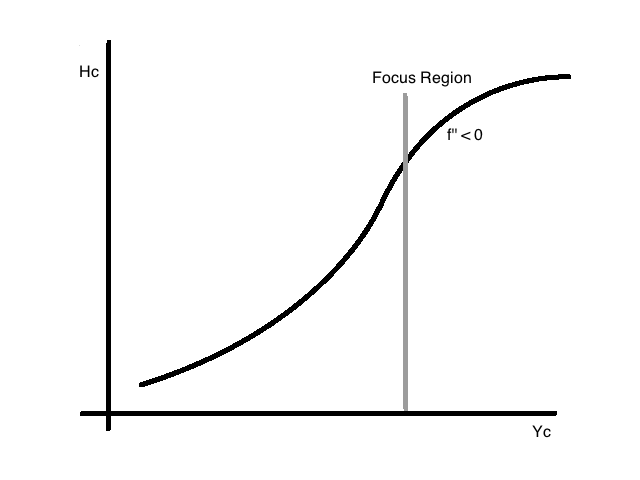
\includegraphics[width=4in, height=3in]{plot1.png}
\end{figure}
\end{center}

You can think of it, by now, in the following way:

\noindent $H_c = f(Y_c, \overline{B})$, where $\overline{B}$ is the ``fixed brain of the kid.'' And, therefore, it is more intuitive that:
\begin{equation*}
\frac{dF (Y_c)}{dy_c} \geq 0 \quad \text{and} \quad \frac{d^2 f(Y_c)}{d y_c^2} \leq 0. \quad (\text{diminishing marginal returns})
\end{equation*}

\vspace{10mm}

\noindent \textbf{Assumption}: All families have same production function.

\begin{itemize}
\item What determines the earnings of the kids?\\
    $W_c = R H_c = R f(Y_c)$ ; $R$ converts human capital into earnings.\\
    $\displaystyle R = \psi (\sum_{t\in T} H_t, \text{ technology}, \text{ physical capital})$
\end{itemize}

\vspace{10mm}

\noindent \textbf{Assumptions}:

\noindent $R$ is constant for each household.\\
$R$ is ``competitive,'' i.e., a household alone can't change it.\\
$R$ is taken by parents as given by the market environment.
%
\begin{itemize}
\item In this model, earnings only differ because of human capital, i.e., by goods spent on children. Gaps may differ by economic sector, but this always holds.
\end{itemize}

\textbf{Economic Problem}

\begin{align*}
\underset{y_c,C_p}{\text{Max}}\ \ &\{ U_p(W_p) = U(C_p) + a\cdot v (W_c)\} \\
&\text{s.t}\ \ C_p + y_c = W_p
\end{align*}

\textbf{Solution}:
\begin{equation*}
\mathcal{L} = U_p(\cdot) - \lambda \left[C_p + y_c - W_p \right]
\end{equation*}

\textbf{F.O.C.'S}:
\begin{equation*}
U'(C_p) = \lambda,\quad a\frac{dV(W_c)}{dy_c}\leq \lambda
\end{equation*}

\begin{itemize}
\item Notice\ \ $W_c = 2 H_c = 2f(y_c)$
\end{itemize}

If $<$ 0, $y^*_{C} = 0$  when?
\begin{itemize}
\item if $a = 0$
\item if income of parents is too low
\end{itemize}

\noindent \textbf{Rewriting}:
\begin{align*}
a \cdot \frac{dV(W_c)}{dW_c} \cdot \frac{dW_c}{dH_c} \cdot \frac{dH_c}{dy_c} \leq 0 &\implies a V' \cdot \underbrace{R f_y}_{\substack{\text{intuition} \\ \text{quetanto un peso} \\ \text{mas de inversion} \\ \text{be ``retorna''}}}  \leq \lambda \\
&\implies \frac{dW_c}{dy_c} = \mathit{l t i} = R_y \\
&; i\ \ \text{marginal rate of return of investment in kids} \\
\end{align*}
\begin{align*}
a V' c \underbrace{R_y}_{\substack{\text{marginal} \\ \text{rate of} \\ \text{return}}} \leq \lambda = U'(C_p) &\implies \underbrace{\frac{U'(C_p)}{a V' c}}_{\substack{\text{HRS of} \\ \text{parents}}} \geq R_y
\end{align*}

If $a > 0$, there is an interior solution: let's assume that parents provide at least food and shelter to kids.

\begin{center}
\begin{figure}[H] 
\caption{}
\centering
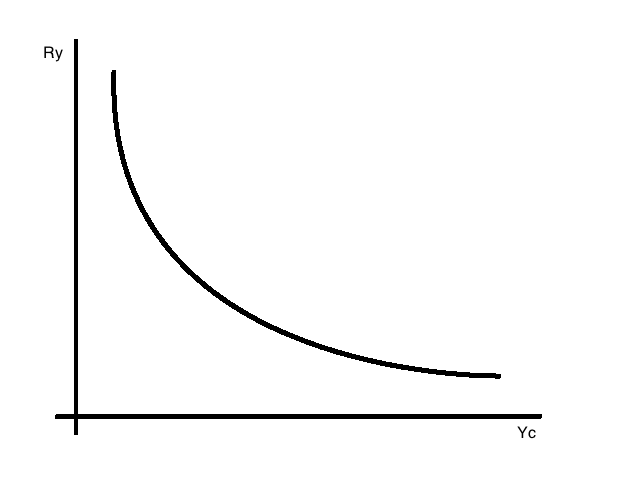
\includegraphics[width=4in, height=3in]{plot2a.png}
\end{figure}
\end{center}

\begin{center}
\begin{figure}[H] 
\caption{}
\centering
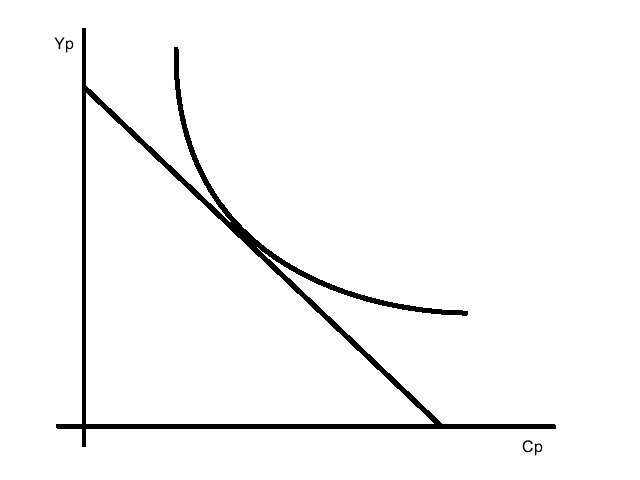
\includegraphics[width=4in, height=3in]{plot2b.png}
\end{figure}
\end{center}

\textbf{Two basic equations}:

\begin{align*}
a r f_y V'_{c} - U'(C_p) = 0 \quad \ldots \quad g_1 (y_c, C_p; a, r, W_p) \\
C_p + y_c - W_p = 0 \quad \ldots \quad g_2 (y_c, C_p; a, r, W_p)
\end{align*}

\begin{itemize}
\item What happens when $W_p$ increases to $y_p$ and to $C_p$?
    \begin{itemize}
    \item What happens to endogenous ``choice variables'' when parameters change, in this case $W_p$?
    \end{itemize}
For notation, let
\begin{align*}
g = \begin{bmatrix}
        g_1 \\
        g_2
    \end{bmatrix} \quad \text{and} \quad x &= (C_p, y_c) \\
                                         g &= (a, r, W_p)
\end{align*}
The general implicit function theorem establishes:
notice, \quad $g_1 = a r f_y V'_{c} (r f(y_c)) - U'(C_p)$
\begin{align*}
\begin{bmatrix}
    \ \ \frac{dC_p}{dW_p}\ \ \\
    \ \ \frac{dy_c}{dW_p}\ \
\end{bmatrix} &= - \begin{bmatrix}
                    \ \ \frac{dg_1}{dc_p} \quad &\frac{dg_1}{dy_c}\ \ \\
                    \ \ \frac{dg_2}{dc_p} \quad &\frac{dg_2}{dy_c}\ \
                  \end{bmatrix}^{-1} \begin{bmatrix}
                                        \ \ \frac{dg_1}{dW_p}\ \ \\
                                        \ \ \frac{dg_2}{dW_p}\ \
                                     \end{bmatrix} \\
              &= - \begin{bmatrix}
                        \ \ -U''(c_p) \quad &a r [f_{yy} V'_c + r f_y f_y V''_c]\ \ \\
                        \ \ 1 \quad &1\ \ \\
                    \end{bmatrix}^{-1} \cdot \begin{bmatrix}
                                                \ \ 0 \ \ \\
                                                \ \ -1 \ \ \\
                                             \end{bmatrix} \\
              &= \frac{-1}{-U''(c_p) - a r [f_{yy} V'_c + r f_y f_y V''_c]}(a r = 0 > 0) \cdot \begin{bmatrix}
                                                                                                    \ \ 1 \quad &a r [f_{yy} V'_c + r f_y f_y V''_c]\ \ \\
                                                                                                    \ \ -1 \quad &-U''(c_p)\ \
                                                                                                \end{bmatrix} \cdot \begin{bmatrix}
                                                                                                    0 \\
                                                                                                    -1
                                                                                                \end{bmatrix} \\
              &= \begin{bmatrix}
                    \ \ \frac{- a r [f_{yy} V'_c + r f_y f_y V''_c]}{0}\ \ \\
                    \ \ \frac{-U''(c_p)}{0}\ \
                 \end{bmatrix} > 0
\end{align*}
Make sense because goods are normal and this change in $W_p$ is an income effect.

\item Intergenerational income mobility: studies relation between parents and children income.
It is said that there exists regression to the mean mobility in this matter:
\begin{align*}
ln\ \ W_c = \alpha + h ln\ \ W_p + \epsilon_c
\end{align*}
if : \quad $h=1$ no regression to the mean \\
$h<1$ regression to the mean \\
$h>1$ regression away from the mean.

    \begin{itemize}
    \item Continuing with the discussion about the previous model $\ldots$
    \end{itemize}
What happens with the specifications of the function $H_c = f(y_c)$. Remember, $W_c = r f(y_c)$, and we are supposing $r$ is competitive.
If $f_{yy} = 0$, suppose $H_c = K y_c ; K \in R_{++}$. The situation with the rate of return is the following. We saw the rate of return is $R_y = r f_y$. In this case $f_y = K$, so $R_y$ is the same for all the families, $rK$.
This means that ``capital markets are working perfectly''.
    \begin{itemize}
    \item Now, imagine we have $f_{yy} < 0$. E.g. $k y_c$ with $r < 1$. Then, $R_y = r f_y$ and $\frac{dR_y}{dy} = r f_{yy} < 0$.
    \end{itemize}
In this case, there is an inefficiency: parents can't lend to other poor kids. There is a ``price effect'', diminishing returns on investment: ``invest more rises the cost of investing''. Graphically :

\begin{center}
\begin{figure}[H] 
\caption{}
\centering
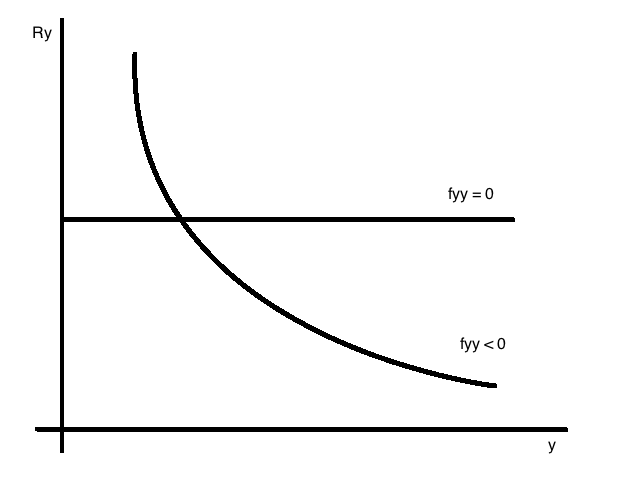
\includegraphics[width=4in, height=3in]{plot3.png}
\end{figure}
\end{center}


$R^{*}_y (\text{poor}) > R^{*}_y (\text{rich})$. Rates of return are different and there is no ``lending access''. Capital markets are not working perfectly.

    \begin{itemize}
    \item returning to the intergenerational income mobility aspects. Take the regression $ln W_c = \alpha + h ln W_p + 2 c$. Since we prove that $\frac{dy_c}{dW_p} > 0$, then it should be clear that $\frac{dW_c}{dW_p} > 0$, so $h > 0$. But, what happens with regression to the mean:

\begin{center}
\begin{figure}[H] 
\caption{}
\centering
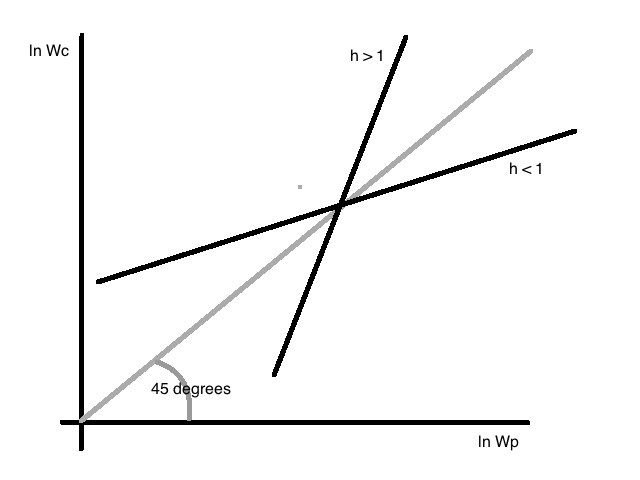
\includegraphics[width=4in, height=3in]{plot4.png}
\end{figure}
\end{center}


    \item In this context, regression to the mean means that if a parent is an average richer, the kid is also an average reacher but less. The literature says that $h \approx .5 - .b$.
    \end{itemize}

What happens with poverty? Take the variance as a measure of poverty. Then $\text{VAR}(ln W_c) = h^2 \text{VAR}(ln W_p) + \text{VAR}(2)$. 

In equilibrium, $\text{VAR}(ln W_c) = \text{VAR}(ln W_p) \quad \text{and} \quad \text{VAR}(ln W_c) = \frac{\text{VAR}(V)}{1-h^2}$. If $h = 1$, the poverty process is ``not stationary''.
\item Some people speak about ``underclass''. Born poor, stay poor. At least from one generation to another.

\item It will make a lot of sense to suppose that the human capital of the kids is also depending on the human capital of the parents. That is: $H_c = f(y, H_p)$, where we are going to take $H_p$ as a constant (there is just one overlapping generation). The ``intuitively economic'' assumptions of this process are:
    \begin{align*}
    \frac{dH_c}{dH_p} > 0 \quad \text{or} \quad \frac{df(y_c,H_p)}{dH_p} > 0 \quad \text{and} \quad \frac{d^2f(y_c, H_p)}{dy_c dH_p} > 0
    \end{align*}

Think of this: $H_c = \overbrace{f}^{\text{same for all families}}(\underbrace{y_c}_{\text{choose}}, \underbrace{H_p}_{\text{given by g.parents}})$, different household technology for each individual.
    \begin{itemize}
    \item This is a recursive property:
        \begin{enumerate}[1.]
        \item As a person increases her human capital she affects her late.
        \item Economy's production today depends on how much you start with. This is a process that you build in what you have.
        \end{enumerate}
    \item Recall that diminishing returns to investment in kids, $f_{yy} \leq 0$. (more information, harder and harder to get it given a brain $\overline{B}$).
        \begin{itemize}
        \item \textbf{one special case}: Suppose $H_c = \psi(y_c) H_p; \frac{d\psi(\cdot)}{dy_c} >, \frac{d^2\psi(\cdot)}{dy_{c^2}} \leq 0$. \\
        Let's see an ``economic growth'' consequence of this:
        \item $\underbrace{\frac{dH_c}{dy_c} = \psi_y(\cdot) H_p}_{\text{more investment, more human capital.}}, \underbrace{\frac{d^2H_c}{dy_c dH_p} \psi_y > 0}_{\text{complementarity}}$
            \begin{itemize}
            \item $\frac{H_p}{H_c} = 1 + g_H = \psi(y_c)$, so if you hold $y_c$ constant, growth rate will be constant for the countries.
            \end{itemize}
        \end{itemize}
    \end{itemize}

\item This is saying that poor economies have it difficult to catch up. (inequality maintains itself constant over time, because growth is constant).
\item If we analyse world per capita income, richer countries have not become richer.\\
Now, let's analyse the parental problem with this modification:
\begin{align*}
\underset{c_p,y_c}{\text{Max}} \quad U(c_p) + a V_c (r f(y_c, H_p))\\
[cp] : U'(c_p) = \lambda \quad [y_c] = a \cdot V'_c \cdot r \cdot f_y = \lambda \\
\end{align*}
The first order conditions are the same, but in this case $g = (a, r, W_p, H_p),\ \ x= (c_p, y_c)$. It might be interesting to know what happens when $H_p$ changes. This is:
\begin{align*}
\begin{bmatrix}
    \frac{dc_p}{dH_p} \\
    \frac{dy_c}{dH_p}
\end{bmatrix} = - \begin{bmatrix}
                    \ \ \frac{dg_1}{dc_p} & \frac{dg_1}{dy_c}\ \ \\
                    \ \ \frac{dg_2}{dc_p} & \frac{dg_2}{dy_c}\ \
                  \end{bmatrix}^{-1} \begin{bmatrix}
                                        \frac{dg_1}{dH_p} \\
                                        \frac{dg_2}{dH_p}
                                     \end{bmatrix}\\
\end{align*}
Notice,
\begin{align*}
a r f_y(y_c, H_p) V'_c (r f(y_c, H_p)) - U'(c_p) &= 0 \quad \ldots \quad g_1 \\
c_p + y_c - W_p &= 0 \quad \ldots \quad g_2 \\
\end{align*}
\begin{align*}
\begin{bmatrix}
    \frac{dg_1}{dH_p} \\
    \frac{dg_2}{dH_p}
\end{bmatrix} = \begin{bmatrix}
                    \ \ a r [f_{yH} V'_c + f_y \cdot V''_c \cdot r f_H]\ \ \\
                    \ \ 0\ \
                \end{bmatrix} \\
\end{align*}
Set $\frac{dW_p}{dH_p} = r = 0$ by taxing. ; $W_p = r H_p = r f (y_p)$
\begin{align*}
\begin{bmatrix}
\frac{dc_p}{dH_p} \\
\frac{dy_c}{dH_p}
\end{bmatrix} &= \frac{-1}{0} \begin{bmatrix}
                                \ \ 1 & - a r (f_{yy} V'_c + r f_y f_y V''_c)\ \ \\
                                \ \ -1 & -V''(c_p)\ \
                             \end{bmatrix} \cdot \begin{bmatrix}
                                                    a r [f_{yH} V'_c + f_y V''_c r f_H] \\
                                                    0
                                                 \end{bmatrix} \\
              &= \begin{bmatrix}
                    \frac{\overbrace{-a r f_{yH} V'_c}^{(4) < 0} - \overbrace{a r f_y V''_c r f_H}^{> 0 (3)}}{0} \\
                    \overbrace{+ (\underbrace{a r f_{yH} V'_c}_{>})}^{> 0 (2)} \overbrace{+ (\underbrace{a r f_y V''_c r f_H}_{<})}^{< 0 (1)}
                 \end{bmatrix} \ldots \text{can't sign} \\
\end{align*}

$\frac{dy_c}{dH_p}$ \quad : (1) ``Income effect'' (feels reacher because $H_p$ increases), consume more for himself. Since the budget constraint is fixed, ``eat more for me, as parent''. \\
$\frac{dy_c}{dH_p}$ \quad : (2) ``Substitution effect'' (changing the prices of investing) pushing you to invest more on kid capital \\
$\frac{dc_p}{dH_p}$ \quad : reversed.
\end{itemize}

\begin{itemize}
\item This is why the question, do more educated parents spend more time $(y_c)$ with their kids?, remains unclear theoretically.
\item Empirically, measuring the magnitude of the ``income effect'' and the ``substitution effect'', more educated parents spend more time $(y_p)$ with their kids.
\item Two properties of ``kids markets'' are the following:\\
(recall $f(y,H_p)$ and $f_y >0, f_{yy} <0$).
    \begin{itemize}
    \item you \textbf{do affect} them when you give them things (towards negating competition)
    \item every household is having its own production function. \\
    \end{itemize}
Think: $H_c = f(y_p, y_c, H_{gp})$, and so on $\ldots$
\end{itemize}

\textbf{Equity v.s. efficiency}:

If $H_c= f(y_c)$: 

There is no trade-off between efficiency and equity: go ahead and give to the poor \\
because they have more $R_y$.

\begin{center}
\begin{figure}[H] 
\caption{}
\centering
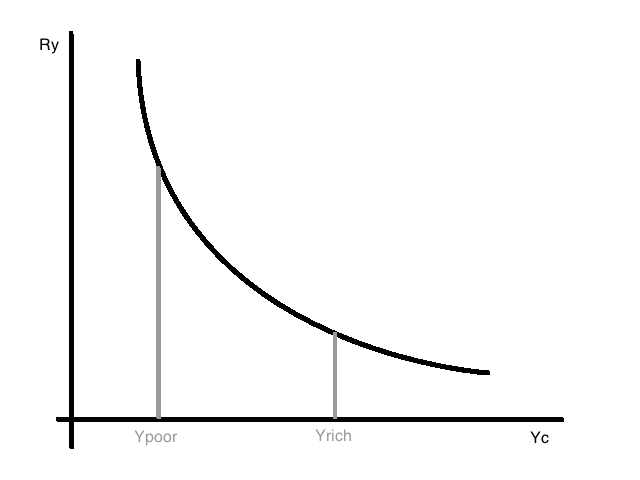
\includegraphics[width=4in, height=3in]{plot5.png}
\end{figure}
\end{center}


If $H_c = f(y_c, H_p)$:
\begin{itemize}
\item For g, it is more efficient $y_c$ spending for the rich, but this varies across different $y's$.
\end{itemize}

\begin{center}
\begin{figure}[H] 
\caption{}
\centering
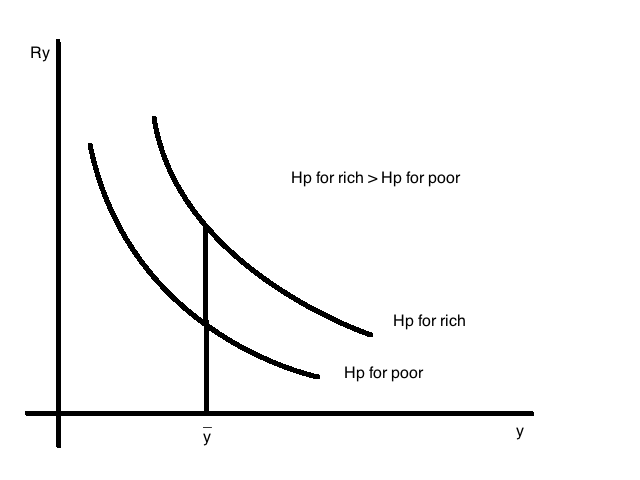
\includegraphics[width=4in, height=3in]{plot6.png}
\end{figure}
\end{center}


\textbf{Ability} (may be important in regression to the mean)

\begin{itemize}
\item How to introduce ability:
\begin{align*}
A_c = (1-h) \overline{A} + h A_p + V_c \quad E[V_c] = 0 \quad E[A_c] = E[A_p] = \overline{A}
\end{align*}
$h \rightarrow$ degree of inheritability: \quad $0 \leq h \leq 1$.
\end{itemize}


In our analysis we assume there is a single dimension abilities and is early determined.
\begin{itemize}
\item Why is ability important?
    \begin{itemize}
    \item determines inequality (e.g. earnings in cohort)
    \item intergenerational mobility
    \end{itemize}
\end{itemize}

\textbf{Bring in abilities}: \quad $H_c = f(y_c, H_p, A_c); \quad \frac{df}{dA_c} = f_A > 0$
\begin{itemize}
\item If you are more able investment is better for you: $f_{yA} \geq 0$
\item $df_{HA}?$ not going to work much.
    \begin{itemize}
    \item What happens if $A_c$ raises?
    \end{itemize}
\begin{align*}
&\frac{dW_c}{dA_c} > 0 \quad \frac{dH_c}{dA_c} > 0, \quad \text{but} &\frac{dy_c}{dA_c} < 0 \quad \text{income effect} \\
&R_y = r f_y \quad \text{raises} &\frac{dy_c}{dA_c} > 0 \quad \text{substitution effect}
\end{align*}
\item You can't sign neither $\frac{dc_p}{dA_c}$.
\end{itemize}

\textbf{Intergenerational perspective}

Parental ability: \quad $\frac{dW_p}{dA_p} > 0, \quad \frac{dH_p}{dA_p} > 0$.
\begin{itemize}
\item Ability increases means more earning and more human capital.
\item Higher ability of parents will increase $H_c$  of child through effect on income on $H_p$ of parents (indirect channel). There may also be a direct channel. Assume a transmission mechanism:
\begin{align*}
A_c = \underbrace{(1-h) \overline{A}}_{\substack{\text{average ability} \\ \text{of society}}} + h A_p + V_c \\
\end{align*}
$h$, degree of inheritability of adult to child \\
$V_c$, random determinant of ability of child. (independent across generations and individuals). \\
If $0<h<1$, regression to the mean. \\
If $h=0$, ability is just random. \\
In equilibrium, $\text{VAR}(A_c) = r^2 A_c = r^2 A_p = r^2 A = \text{VAR}(A_0)$, then \\
$\text{VAR}(A_c) = h^2 \text{VAR}(A_p) + \text{VAR}(V_c) \implies \text{VAR}(A^*) = \frac{\text{VAR}(V_c)}{1 - h^2}$. Note $\frac{1}{1-h^2}$ multiplier.
\item We want to link this to earnings in two situations:
    \begin{itemize}
    \item perfect capital markets
    \item imperfect capital markets
    \end{itemize}
\item Recall $H_c = f(y_c, A_c)$ and assume perfect capital markets. \\
This means ${R_y}^* = R$ for all families:
\end{itemize}

\begin{center}
\begin{figure}[H] 
\caption{}
\centering
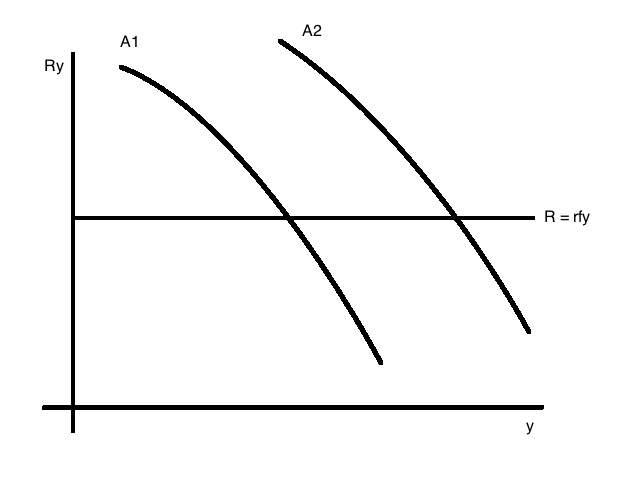
\includegraphics[width=4in, height=3in]{plot7.png}
\end{figure}
\end{center}

everyone will have the same $rf_y$ around this point.\\
Let's say two persons have $A_1$, but they have different incomes, say $W_{p Low}, W_{p High}$. This will cause borrowing-repayment situations.


\textbf{Perfect capital model}

If capital market are perfect, the income of the child will only depend on his ability:
\begin{equation}
W_c = a + b A_c + V_c
\end{equation}
\begin{equation}
W_p = a \quad b A_p + V_p
\end{equation}
\begin{equation*}
\Leftrightarrow b A_p = W_p - a - V_p
\end{equation*}
And we know that the ability process is:
\begin{align*}
A_c = (1-h)\overline{A} + h A_p + \epsilon_c
\end{align*}
Then
\begin{align*}
W_c = a + b[(1-h)\overline{A} + h A_p + \epsilon_c] = a + b(1-h)\overline{A} + b h A_p + b \epsilon_c \\
\end{align*}
So
\begin{align*}
W_c &= a + b(1-h)\overline{A} + h[W_p - a - V_p] + b\epsilon_c \\
W_c &= a + b(1-h)\overline{A} + hW_p - ah - hV_p + b\epsilon_c \\
W_c &= \underbrace{a + b(1-h)\overline{A} - ah}_{c} + hW_p - \underbrace{h V_p + b \epsilon_c}_{\theta c} \\
\end{align*}
Then $W_c = c + h W_p + \theta_c$, which depicts that $W_p$ is a ``perfect signal'' of $A_c$ when capital markets are perfect.

\textbf{Imperfect capital markets model}

\begin{align*}
ln A_c &= a + h ln A_p + V_c; \quad ln \overline{A_c} = ln \overline{A_p} = ln \overline{A}, \\
ln A_c &= (1-h) ln \overline{A} + h ln A_p + V_c \\
ln W_c &= b + c ln W_p + \epsilon
\end{align*}
\begin{itemize}
\item $ln W_c = \alpha + \beta ln A_c + \gamma ln W_p$
\end{itemize}

\textbf{Substitutions ln $A_c$}:
\begin{itemize}
\item $ln W_c = \alpha + \beta (1-h) ln \overline{A} + \beta h ln A_p + \gamma ln W_p$
\end{itemize}
but we know:
\begin{align*}
ln W_p &= \alpha + \beta ln A_p + \gamma ln W_{GP} \\
\Leftrightarrow \beta ln A_p &= ln W_p - \alpha - \gamma W_{GP}
\end{align*}
Then
\begin{align*}
ln W_c &= \alpha + \beta (1-h) ln \overline{A} + h ln W_p - h \alpha - h \gamma ln W_{GP} + \beta V_c + \gamma ln W_p \\
&= (1-h)(\alpha + \beta ln \overline{A}) + (h+\gamma)ln W_p - \underbrace{h \gamma ln W_{GP}}_{\text{Why?}} + \beta V_c \\
\end{align*}

\begin{itemize}
\item Why impact of $W_{GP}$ is negative? \\
Recall $-h \gamma$ is a coefficient that holds everything else constant. \\
Suppose there are two persons, $1$ and $2$:
\begin{align*}
&1 \quad &2 \\
&W_0 &W_0 \\
&\uparrow A_p &A_p \downarrow \\
&\downarrow y \implies W_{GP}\downarrow &\uparrow y \implies W_{GP}\uparrow\\
\end{align*}
\begin{align*}
ln W_p = \alpha + \beta ln A_p + \gamma ln W_{GP}\\
\end{align*}
If $W_p$ is fixed, when someone has more $W_p$ she has less $A_p$.
\end{itemize}

\textbf{Now, we can model this including the human capital of the parents}:
\begin{align*}
ln A_c &= (1-h)ln \overline{A} + h ln A_p + V_c \\
ln W_c &= \alpha + \beta ln A_c + \gamma ln W_p + \delta ln H_p; \quad r H_p = W_p \Leftrightarrow ln r + ln H_p = ln W_p \\
ln W_c &= \alpha + \beta ln A_c + \gamma ln W_p - \delta ln r + \delta ln W_p \\
ln W_c &= \alpha + \beta ln A_c + (\gamma+\delta) ln W_p - \delta ln r \\
&\Leftrightarrow ln W_p = \alpha + \beta ln A_p + (\gamma+\delta) ln G_P - \delta ln r \\
&\Leftrightarrow \beta ln A_p = ln W_p - \alpha - (\gamma+\delta) ln G_P + \delta ln r \\
\end{align*}
\begin{align*}
ln W_c &= \alpha + \beta \big[ (1-h) ln \overline{A} + h ln A_p + V_c \big] + (\gamma+\delta) ln W_p - \delta ln r \\
&= \alpha + \beta(1-h) ln \overline{A} + \beta h ln A_p + \beta V_c + (\gamma+\delta) ln W_p - \delta ln r \\
&= \alpha + \beta(1-h) ln \overline{A} + h \big[ ln W_p - \alpha - (\gamma+\delta) ln W_{GP} + \delta ln r \big] + (\gamma+\delta)lnW_p - \delta lnr \\
&= \alpha + \beta(1-h) ln \overline{A} + hln W_p - h\alpha - h(\gamma+\delta) ln W_{GP} + h\delta ln r + (\gamma+\delta)lnW_p - \delta lnr \\
ln W_c &= \alpha + \beta(1-h) - h\alpha + (h+\gamma+\delta)ln W_p - h(\gamma+\delta) ln W_{GP} + \delta(h-1) ln r. \\
\end{align*}

\textbf{Returning to our household production problem}

\begin{itemize}
\item Another question that might be interesting is if there is more than one child, what happens? \\
\textbf{Motivation}: Consider the abilities of the two childs $A_1, A_2$ with $A_1 > A_2$.
\begin{align*}
H_c = f(y_c, A), \quad \text{with} \quad f_{yc} > 0, \quad f_A > 0, \quad f_{y} \cdot A > 0. \\
\end{align*}
What happens with $y^*_1$ and $y^*_2$. Clearly, efficiency establishes $y^*_1 > y^*_2$.
\item If $H^*_1 = H^*_2$, then $W_1 = W_2 = r H$ only possible if $y^*_1 < y^*_2$. The parent is a social planner inside his family.
\end{itemize}

\textbf{Natural generalization}

$U(W_p) = U(c_p) + a_1 V_1 (Wc_1) + a_2 V_2 (Wc_2)$, we can assume both $a_1 = a_2$ and $V_1 = V_2$.
\begin{itemize}
\item Perfect capital market which implies $R^*_1 = R^*_2 = R$ which implies $y^*_1 > y^*_2 \implies H^*_1 > H^*_2 \implies V^*_1 > V^*_2$.
\item The problem is:
\begin{align*}
U(W_p) &= U(c_p) + a_1 V_1 (Wc_2) + a_2 V_2 (Wc_2) \\
Wc_1 &= r H_{c1} = r f_{c1} \quad H = f(y_c) \\
W_2 &= r H_{c2} = r f_{c2} \\
\end{align*}

\begin{center}
\begin{figure}[H] 
\caption{}
\centering
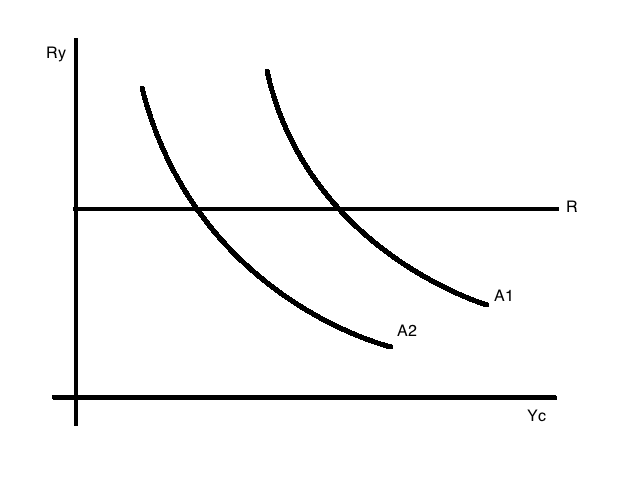
\includegraphics[width=4in, height=3in]{plot8.png}
\end{figure}
\end{center}

budget constraint of parents: $c_p + y_1 + y_2 = W_p$

\textbf{First order conditions}

\begin{align*}
U'(c_p) = \lambda = \underbrace{a_1 \frac{dV_1}{dy_1} = a_2 \frac{dV_2}{dy_2}}_{\substack{\text{last dollar spent in} \\ \text{each kids gives the} \\ \text{same utility for parents}}} \\
\Rightarrow a_1 V'_1 r f_{yz} = a_2 V'_2 r f_yz \Leftarrow \\
\text{if} \quad a_1 = a_2 = a, \quad \text{then} \underbrace{V'_1 r f_{y_1} = V'_2 r f_{y_2}}_{\substack{\text{last dollar spent in} \\ \text{each kids gives the} \\ \text{same utility for parents}}} \\
\end{align*}

\item Could it be in equilibrium that $V^*_1 < V^*_2$? \\
If this is true, $V'_1 < V'_2$, then $f^*_{y_1} < f^*_{y_2}$. This means $y^*_1 > y^*_2$, which implies $H^*_1 > H^*_2 \Leftrightarrow W^*_1 > W^*_2 \Leftrightarrow V_1 > V_2 \quad \bm{!}$. \\
Then, in equilibrium $V^*_1\geq V*_2$. \\
Parents take compromises balancing their spendings between kids. Degree of concavity of $V'_1$ matters:

\begin{center}
\begin{figure}[H] 
\caption{}
\centering
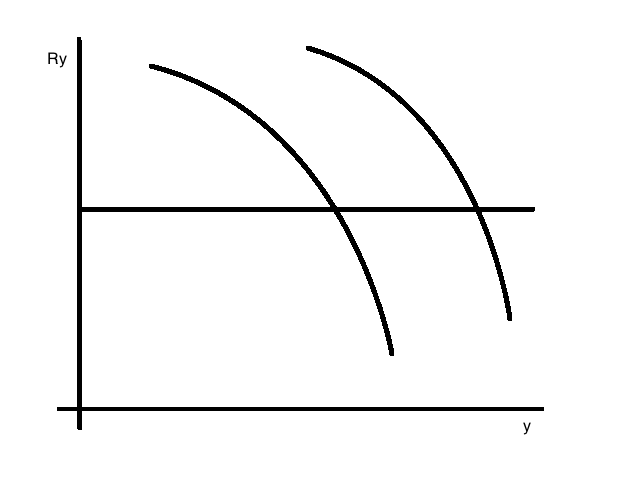
\includegraphics[width=4in, height=3in]{plot9.png}
\end{figure}
\end{center}

$y^*_1 < y^*_2$ possible, but implies $H^*_1 > H^*_2$ because $W^*_1 > W^*_2$ (ability).
\item Since $a_1f_{y1}V'_1 = a_2f_{y2}V'_2$, it is more likely that $y_2 > y_1$ as $\frac{a_2}{a_1}$ increases. \\
In general, $W_{c_1} \neq W_{c_2}$ because rates the return differ by kid.
\item Parents do all the time a trade-off between efficiency and equality as government do with inequality and OWL's that taxes generate.
\item Now, suppose the parents don't know the abilities of the child. Then, ability can be $A_1$ or $A_2$.
\item Suppose Prob($A_1$) = .5 and Prob($A_2$) = .5, this means that the problem of the parents is: \\
The problem that parents face now is:
\begin{align*}
U(W_p) = U(c_p) + .5 a V_1 (A = A_2) + .5 a V_1 (A=A_1) + .5 a V_2 (A=A_2) + .5 a V_2 (A=A_1)
\end{align*}
and they have to choose $c_p,y_1,y_2$. In equilibrium, $y^*_1 = y^*_2$: they will have same expected utility of their investments. (notice that variance may matter as well).
\end{itemize}

\textbf{Other Capital than Human}

Define other form of capital: there is a return from capital that is the same for everyone: $R_k$. What are the consequences for our household production model.

Simplicity: return to the single child household production. We model the situation in which very little $y$ will give very high $R_y$: \\

\begin{center}
\begin{figure}[H] 
\caption{}
\centering
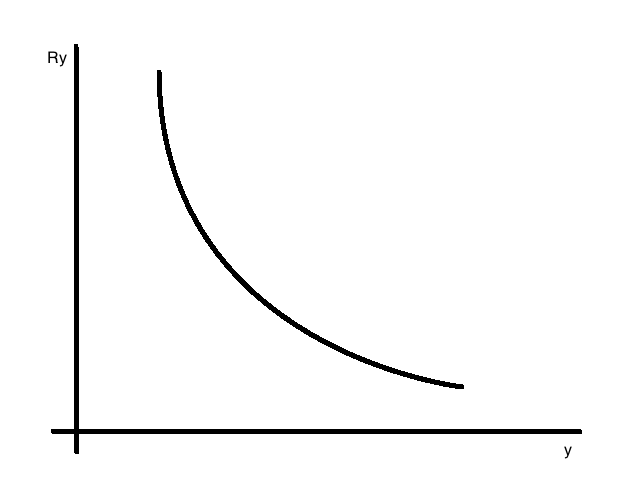
\includegraphics[width=4in, height=3in]{plot10.png}
\end{figure}
\end{center}

\begin{itemize}
\item Very little $y$ gives very high $R_y$. Think: $R_y \to \infty$ as $y \to 0$, so $y > 0$.
\item Every family $y > 0$, as long as $R_y > R_k$, which is a weak assumption.
\item As parents become richer, $R_y < R_k$.
    \begin{itemize}
    \item Now, we are going to consider the income (welfare) of the kid: $I_c = W_c + R_k \cdot K a$
    \item Now, we have two forms of investment, then the parents budget constraint is: $c_p + y_c + k_c = I_p$.
    \item The utility function of the parents now is:
    \end{itemize}
\begin{align*}
U(T_p) = U(c_p) + a V \underbrace{(W_c + R_k K_c)}_{I_c}. \\
\end{align*}
Then, the first order conditions of the problem are:
        \begin{itemize}
        \item $U'(c_p) = \lambda$
        \item $a V'_c \frac{dI}{dy_c} = \lambda$
        \item $a V'_c \cdot \frac{dI}{dK_c} \leq \lambda$, if $<, K_c = 0$.
        \item $a V'_c R_k \leq a V'_c R_y \Leftrightarrow R_k \leq$
        \end{itemize}
\item Corner solution may be possible in $K_c$.
    \begin{itemize}
    \item $\frac{dy*}{dI_p}\big\}\substack{\text{normal} \\ \text{good}}$ \ \ as long as $R_y > R_y$.
    \end{itemize}
\end{itemize}

\begin{center}
\begin{figure}[H] 
\caption{}
\centering
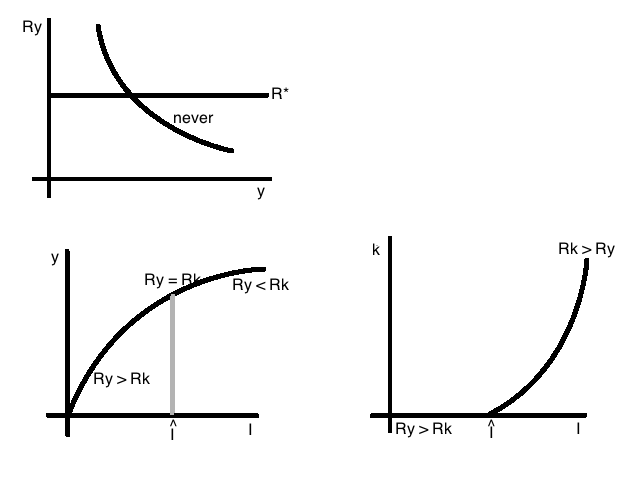
\includegraphics[width=4in, height=3in]{plot11.png}
\end{figure}
\end{center}

\textbf{Household production with an overlapping period when children are adults}

\begin{itemize}
\item Initially, parents can't leave debt to their children.
\item Parents can also invest in other capital rather than the one of their kids.
\item Parents can leave ``bequest'' to their kids.
\item Parents also receive ``bequest'' from grandparents.
\item Ages: middle (m) and old (o).
\end{itemize}

\textbf{Budget Constraint 1}: (middle age constraint)

\begin{align*}
c_m + y_c + k_m = E_p = W_p + b_p; \quad \text{always} \quad b \geq 0.
\end{align*}

\textbf{Budget Constraint 2}: (old age constraint)

\begin{align*}
&c_0 + b_c = R_k \cdot k_m \\
\textbf{Recall}: \quad &W_c = r H_c = r f(y_c); \quad f_y > 0, f_{yy} < 0, \frac{dR_y}{dy} < 0.
\end{align*}

\textbf{Parents' Utility Function}:
\begin{align*}
U[E_p] = U(c_p) + \beta U(c_0) + \beta a V_c (E_c = W_c + bc); \quad &\beta = \text{discount factor on ``old days consumption''}. \\ &\text{(lifecycle degree of discount)}. \\ &\text{a = altruism}. \\
\end{align*}
\begin{align*}
\underbrace{\beta}_{\text{``discount for future''}} \text{vs.} \underbrace{a}_{\text{``discount for altruism''}} \\
\end{align*}
\begin{itemize}
\item \textbf{Recall}: $U' > 0, U'' < 0, V' > 0, V'' < 0$.
\item The first condition of this problem induce the following problem:
    \begin{itemize}
    \item $U'(c_m) = \lambda$ \quad marginal utility of middle age consumption
    \item $\beta \cdot U'(c_0) = \frac{\lambda}{R_k}$ \quad discounted marginal utility of old age consumption
    \end{itemize}
\item Then, $U'(c_m) = R_k \cdot \beta \cdot U'(c_0)$ \quad optimality between consumption
    \begin{itemize}
    \item $\beta a V'_c R_y = \lambda = U'(c_m); \quad y_c > 0$
    \item $\beta a V'_c \leq \frac{\lambda}{R_k}; \quad < \implies bc = 0, = \implies bc > 0$
    \item $\beta R_k a V'_c = \beta a V'_c R_y \Leftrightarrow R_k \leq R_y; \quad < \implies bc = 0, = \implies bc > 0$
    \end{itemize}

If $a V'_c < U'(c_0)$, then $bc = 0$. The more selfish they are, the less bequest they give. $(R_y > R_k)$. \\
It will be more efficient if you can do negative $b_c$. This will imply ${R_y}^* = {R_k}^*$.
\end{itemize}

\textbf{Public policy problem}: \quad there may be very selfish parents:
\begin{align*}
aV'_c < U'(c_0), \text{when} \quad b_c = 0.
\end{align*}

\textbf{``Preference transmission'' model}
\begin{itemize}
\item Suppose kids have a utility function $V_c (E_c, G); \frac{dV_c}{dG} < 0$ where $G =$ guilt.
\item Suppose parents have the following utility function:
\begin{align*}
U_p = U(c_m) + \beta U(c_0) + a \beta V_c(E_c \cdot G)
\end{align*}
\item Assume $G(z_c)$, where $\frac{dG(z_c)}{dz_c} > 0$ and $z_c$ is the expenditure made by parents in making children guilty.
\end{itemize}

\textbf{Budget constraints of the parents}:

\begin{align*}
&c_m + y_c + z_c + k_m = E_p + \overbrace{S_p(G)}^{\text{grandparents ``guilty gift''.}} \text{(middle age)} \\
&c_o + b_c = R_{k} K + s_c(G); \quad s(G) \text{is the child support of the parents and} \quad \frac{ds(G)}{dG} > 0. \\
\end{align*}

You lower kids utility in an special way: they fill obligation to come back and give you money in your old days.
\begin{itemize}
\item \textbf{Notice}: in this case $b_c = 0$, what for you will give them ``bequest'' and then spend for them to come back.
\item There are no ``net welfare conclusions''. You lower their utility but you can spend more if they comeback.
\item If $b_c > 0$, then $z_c = 0$, because otherwise the spendings will be inefficient.
\item If you can avoid buying $z_c$ you will do it: you can sign a contract with your son or daughter:
\begin{align*}
R_z > R_k.
\end{align*}
\item A necessary, but not sufficient condition, for parents spending in $z$ is:
\begin{align*}
R_z > R_k. \\
\end{align*}
    \begin{itemize}
    \item The point of this model is to ``endogenize the preferences''.
    \end{itemize}
\end{itemize}

\textbf{More Traditional Human Capital Problem: Education}

This studies the investment of young adults in theirselves. They take as given $H^{\circ}$, the Human capital they have until the period they decide whether or not to go into college. $H_0$, of course is different for every adult.
\begin{equation*}
\left.\begin{aligned}
        \textbf{Life}: \quad &E_{Hi} ; \quad i = 1, \ \ \ldots\ \ , M \\
        &E_{ci} ; \quad i = 1, \ \ \ldots\ \ , M
      \end{aligned}
\right\}
\qquad \text{earning per period in each situation} \\
\end{equation*}

\begin{itemize}
\item College tuition : $f \cdot \quad R = \frac{1}{1+r}$; rate of discount.
\begin{align*}
V_H = \sum \limits_{i=0}^{H} E_{iH} R^{i} \quad &\text{total earnings if stay just with high school}. \\
V_c = \sum \limits_{i=0}^{H} E_{ic} R^{i} - f \quad &\text{total earnings if going to college}
\end{align*}
\end{itemize}

\begin{itemize}
\item If just stay with high school:
\begin{align*}
&E_{OH} = W_{OH} T \\
&E_{OH} = W_{OH} \big[ T - t_c \big]; t_c = \text{time in college}
\end{align*}
\item In $H=0$, both get the same payment.
\item So the point is to compare what happens when you go to high school to what happens when you go to college. \\
    \begin{itemize}
    \item This comparison may be done by the following equation:
    \begin{align*}
    \sum \limits_{i=1}^{M} T \Delta W_i R_i \quad \framebox[1.1\width]{?} \underbrace{T_c W_o}_{\text{forgone earnings}} + \underbrace{f}_{\text{tuition}}
    \end{align*}
    Notice that $\Delta W_i = W_{ci} - W_{Hi}$, is the wage differential of ``college to high school'' and the equation assumes that:
    \begin{align*}
    \Delta W_i = \Delta W_j \quad \forall\ \ i, j
    \end{align*}
    \end{itemize}
\item There are six relevant parameters in the study of this decision:
    \begin{itemize}
    \item $T_c$ = hours of college.
    \item $W_0$ = wage at $t=0$, which is the same for both high school and college.
    \item $H$ = life expectancy
    \item $\Delta W$ = ``benefits of college''
    \item $W_0 T_c$ = forgone earnings
    \item $f$ = tuition
    \end{itemize}
\item Now, if we consider the complete serie:
\begin{align*}
\sum \limits_{i=1} T \Delta W_i R_i = T \Delta W \cdot [\frac{1 - R^{M+1}}{1 - R}] \quad \framebox[1.1\width]{?} \quad f + T_c \cdot W_o
\end{align*}
    \begin{itemize}
    \item This analysis can be extended to ``add'' the probability of dying at age $i$., which will be different in each period of the agent's life. So if we let $m_i$ be this probability:
    \begin{align*}
    \sum \limits_{i=1}^{M} T (1-m_i) \Delta W_i R_i \quad \framebox[1.1\width]{?} \quad f + T_c \cdot W_o
    \end{align*}

    \item Suppose, for a conceptual exercise, that there is no tuition. Then, a flat tax to earnings will not affect the decision. (i.e. the term $(1-\tau)$ will drop out).

    \item If there is tuition, on the other hand, costs are falling by less than $\tau$ and the costs are less (i.e. the decision may be affected).

    \item Clearly, ability affects both: forgone earnings and wage differentials. We can think of this cancelling out on both sides of the equation.
    \end{itemize}
\end{itemize}

\textbf{Why do we have this large increases in tuition?}

\begin{itemize}
\item Education is intensive in education
\item I.e.: increase in tuition is due to increase an increase in costs. Large tuition is related to higher returns to college.
\item Then, it should be true that the following inequality holds:
\begin{align*}
\frac{d(\frac{W_c}{W_H})}{dt} > 0.
\end{align*}
\end{itemize}

\textbf{Think of inequality}: ``Why is there no more people taking advantage of ``college premium''.
\begin{itemize}
\item Dropout high school: face awful situation in any dimension:
    \begin{itemize}
    \item employment
    \item earnings
    \item wealth
    \item marriage (less getting, more divorced).
    \end{itemize}
    \framebox[1.1\width]{Note: Accumulation of capital also explains rise in wages}
\item Now, let's say there is a set of abilities: \\
$A$ = abilities (cognitive and non-cognitive) \\
$H_o$ = initial Human Capital at high-school graduation. \\
If we want to ``endogenize'' time spent in college, what are some reasonable assumptions:
\begin{align*}
T_c (A, H_o); \quad \frac{dT_c}{dA} \leq 0, \quad \frac{dT_c}{dH_o} \leq 0 \\
\end{align*}
Also, we can consider the determinants of ``tuition fees'':
\begin{align*}
&f(A, H_o); \quad \text{where}\ \ f \text{are tuition fees}. \\
&\text{Then}, \quad \frac{df}{dA} < 0 \quad \text{and} \quad \frac{df}{dH_o} < 0.
\end{align*}
    \begin{itemize}
    \item The wage differential can be signed here as well:
    \begin{align*}
    \Delta W^{k} (R^{k}, A^{k}, H^{k}_o, M^{k}, T^{k}); \quad \text{k is an individual}.
    \end{align*}
    \item $\frac{d\Delta W^{k}}{dR} < 0 \quad \frac{dW^{k}}{dt_c} > 0$.
    \end{itemize}
Empirically, education gains are everywhere:
    \begin{itemize}
    \item less marriage brokes
    \item better health
    \item raise productivity in household production
    \item better use of contraception methods
    \item better use of drugs
    \item better adaptation of new environments (e.g. technology)
    \end{itemize}
\end{itemize}

\textbf{Model education with Utility}:

We model the individual's utility as one given by the following function:
\begin{align*}
U(x_i, l_i, H, s_i); \quad i = 1,2
\end{align*}
where $x$ = goods \quad $l$ = leisure \quad $s$ = college \quad $m$ = hours worked \\
$t$ = tuition fees \quad $T$ = total time = 1 \\
$h$ = hours spent in investing in college \\
$H$ = high school education \\
Then:
\begin{align*}
l_1 + m_1 + h = T \quad \text{and} \quad l_2 + m_2 = T.
\end{align*}
The ``total'' utility function is: \\
$V = U_1(x_1, l_1, H) + p(H,s) \beta U_2(x_2, l_2, H, s)$, where $p(\cdot)$ is the probability of surviving in period $2$ and $p$ is the discount rate.

\textbf{In this kind of models we implicitly assume that there is a ``perfect annuity market'': expected consumption = expected earnings (access to full earnings wherever)}

\textbf{Budget Constraint}:

\begin{align*}
&x_1 + \frac{p(\cdot)\cdot x_2}{1+r} + w_1 l_1 + \frac{p(\cdot)\cdot W_2(\cdot)l_2}{1+r} + f + W_1 h
&= \underbrace{W_1 + \frac{p \cdot W_2 (\cdot)}{1+r} + \frac{p \cdot (s)}{1+r}}_{\text{full income}}
\end{align*}

\textbf{Think}: \quad $s = f(h, H, A_c, A_n); f_j > 0$ with $j = H, A_c, A_n f_{jy}$ for $j \neq y$

\textbf{F.O.C.}

\begin{align*}
U_1 x = \lambda \quad \text{and} \quad \beta U_2 x p = \frac{\lambda_p}{1+r} \\
\text{Suppose that, in equilibrium}, \quad \beta = \frac{1}{1+r}, \quad \text{then}: \quad U_{1x} = U_{2x} \\
\text{Also}: \quad U_{1l} = \lambda W_1 \quad \text{and} \quad p \beta U_{2l} = \frac{\lambda_l W_2}{1+r} \\
\text{then}: \frac{U_{1l}}{\beta U_{2l}} = \frac{W_1}{W_2} (1+r). \quad \text{Likewise, if } \beta = \frac{1}{1+r}, \quad \text{then} \quad \frac{U_{1l}}{U_{2l}} = \frac{W_1}{W_2}.
\end{align*}

\textbf{Increase earnings}:

Increase in tuition (80's and 90's):

\begin{center}
\begin{figure}[H] 
\caption{}
\centering
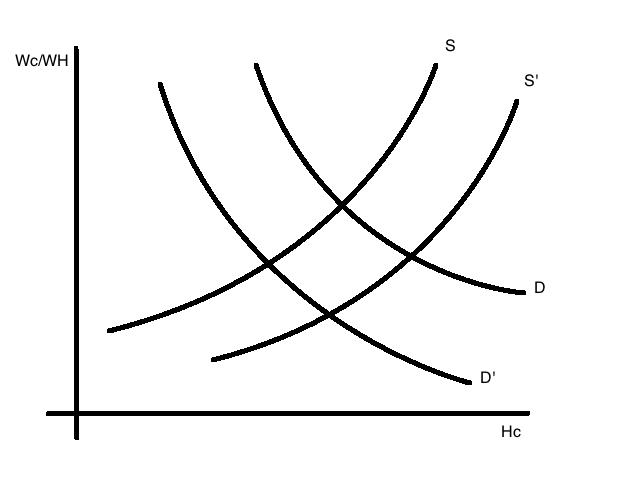
\includegraphics[width=4in, height=3in]{plot12.png}
\end{figure}
\end{center}

\begin{itemize}
\item Education not only gives you skills, it gives you ``techniques'' to know how to ``get information'': learning how to learn. (Schooling is an effective way to do this).

\item Information acquisition aspects

\item Efficient way to get social networking
\end{itemize}

\textbf{Health as Human Capital}

\begin{itemize}
\item We want to treat health as investment per se.
\item Mechanical medicine (surgery instruments) and people's decisions of health
\item We want to study ``what people do with their health''.
\end{itemize}
In an ordered fashion:
\begin{enumerate}[1.]
\item Statistical value of life (SVL)
\item Optimal investment in health
    \begin{enumerate}[a.]
    \item health as self protection
    \end{enumerate}
\end{enumerate}

The ``utility maximizing problem'' is:
\begin{align*}
&\underset{x_1, l_1, x_2, p_2, h}{MAX} \quad U(x_1,l_1) + \beta s(h, \text{schooling})\ \ U(x_2, l_2) \\
&\text{s.t.} \quad x_1 + \frac{s(h)x_2}{1+r} + g(h) = W_1 (1-l_1) + \frac{s(h,\text{schooling})\cdot W_2 (1-l_2)}{1+r}
\end{align*}
\framebox[1.1\width]{Total time = 1} \quad $x_i \rightarrow$ consumption \quad $p \rightarrow$ discount factor \quad $l_i \rightarrow$ leisure

Basic assumptions:
\begin{align*}
g' = \frac{dg()}{dh} > 0 \quad g'' \geq 0, \quad \text{convex cost function} \\
s' = \frac{ds(\cdot)}{dh} > 0 \quad s'' \leq 0, \quad \text{diminishing marginal returns}
\end{align*}

\textbf{First order conditions}:
\begin{align}
[x_1]: U_{x1} (x_1, l_1) &= \lambda \label{eq:1} \\
[x_2]: \beta s() U_{x2} (x_2, l_2) &= \frac{\lambda s(\cdot)}{1+r} \\
[l_1]: U_{l1} (x_1, l_1) &= \lambda W_1 \label{eq:3} \\
[l_2]: \beta s(\cdot) U_{l2} (x_2, l_2) &= \frac{\lambda \cdot s(\cdot) W_2}{1+r} \\
[h]: \beta s'(\cdot) U(x_2, l_2) &= \lambda [g'(\cdot) + \frac{s'(\cdot)}{1+r} (x_2 - W_2(1-l_2))] \label{eq:5}
\end{align}
From \ref{eq:1} and \ref{eq:3}: $\frac{U_{l1}(x_1,l_1)}{U_{x1}(x_1,l_1)} = W_1$

Assumption: persons discounts in the same way than the market. \\
Then: $\frac{U_{x2}(x_2,l_2)}{U_{x1}(x_1,l_1)} = 1$

To analyze \ref{eq:5}, we can make a ``Math Commercial''.

\textbf{Define}: an homogeneous function of degree $k$ is:
\begin{align*}
f(\alpha x) = \alpha^{k} \cdot f(x).
\end{align*}

If $U$ is b.o.d $\gamma$, then $U(\alpha x, \alpha l) = \alpha^{\gamma} \cdot U(x,l)$.

If $\gamma = 1$, the function is ``linear''
   $\gamma < 1$,                 ``concave''
   $\gamma > 1$,                 ``convex''

\begin{center}
\begin{figure}[H] 
\caption{}
\centering
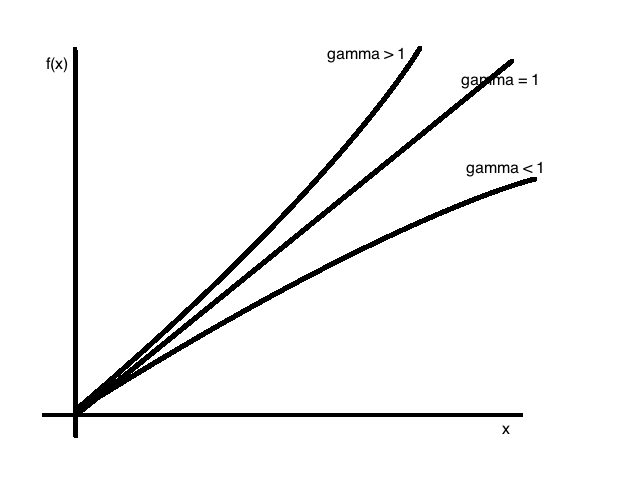
\includegraphics[width=4in, height=3in]{plot13.png}
\end{figure}
\end{center}

\textbf{Euler's theorem}:

Take $x,l$ and define $x' = tx$ and $l'=tl$, then $U(x',l') = t^{\gamma}\cdot U(x,l)$ because $U$ is b.o.d of degree $\gamma$.

Taking the derivative with respect to $t$ of each side:
\begin{align*}
\frac{dU}{dx'}\cdot \frac{d(t_x)}{dt} + \frac{dU}{dl'} \cdot \frac{d(tl)}{dt} = \gamma t^{\gamma - 1} \cdot U(x,l) \\
\Leftrightarrow U_x(tx, tl) \cdot x + U_o(tx,tl)\cdot l = \gamma \cdot t^{\gamma-1} \cdot U(x,l)
\end{align*}
If t = 1:
\begin{align*}
U_x(x,l)\cdot x + U_l \cdot (x,l)\cdot l = \gamma \cdot U(x,l)
\end{align*}
Then:
\begin{align*}
\frac{1}{\gamma}[U_x(x,l)\cdot x + U_l \cdot (x,l)] = U(x,l).
\end{align*}

We can take \ref{eq:5} and substitute $\lambda = U_{x2}(x_2,l_2)$:
\begin{align*}
\beta \cdot s'() \cdot U(x_2, l_2) = U_{x2} (x_2, l_2) [g'(\cdot) + \frac{s'(\cdot)}{1+r} (x_2 - W_2(1-l_2))]
\end{align*}
Recalling that $\beta = \frac{1}{1+r}$, then:

\begin{align*}
\frac{s'(\cdot)}{1+r} \cdot \frac{U(x_2,l_2)}{U_{x2}(x_2,l_2)} = \framebox[1.1\width]{$g'(\cdot) + \frac{s'(\cdot)}{1+r} (x_2 - W_2 (1-l_2))$} \rightarrow \quad \text{RHS}
\end{align*}

\framebox[1.1\width]{If $U$ is b.o.d $\gamma$, then $\frac{U(x_2,l_2)}{U_{x2}(x_2,l_2)} = \frac{1}{\gamma} (U_x \cdot x_2 + \underbrace{\frac{Ul^2}{Ux^2}}_{WL} \cdot l_2)$}

Then
\begin{align*}
\frac{s'(\cdot)}{1+r} \cdot \frac{1}{\gamma} \cdot (x_2 - w_2 l_2) = RHS
\end{align*}
or:
\begin{align*}
s'(h) \cdot \frac{1}{\gamma} (x_2 - W_2 l_2) - \frac{s'(\cdot)}{1+r} (x_2 - l_2 w_2) = g'(\cdot) + (-W_2) \cdot \frac{s'(\cdot)}{1+r}
\end{align*}
Then:
\begin{align*}
\frac{s'(h)}{1+r} [ \frac{1}{\gamma}-1 ] (x_2 + W_2 l_2) = g'(\cdot) + \frac{s'(\cdot)}{1+r} (-W_2).
\end{align*}

\textbf{Statistical Value of Life}

\textbf{Tipical Literature}: \quad Money value of MAN.
\begin{itemize}
\item Tipical income in US $\$40,000$
\item Take 1.8 of that for maintenance and leisure: $\$72,000$
\item Annual value $\$110,000$, but missing the value of $\gamma$. Let's say it is $\gamma = y_2$.
\item Then $W = 2(110,000) = 220,000$.
\item If the discount rate is $4\%$, then:
\begin{equation*}
VSL = \frac{220,000}{.04} = \$5,500,000 \quad \text{in the U.S.}
\end{equation*}
\end{itemize}

\textbf{Exercise}
\begin{itemize}
\item How costly was the $AH_1N_1$ flu in Mexico:

GDP per capita in Mexico: $\$13,500$

Number of deaths $119$

VSL = $5,500,000 \cdot \frac{13,500}{40,000} = 1,856,250$

Stat.loss = $119(1,856,250) = 220,893,750$

\item What about Haiti earthquake

GDP per capita Haiti: $\$1,300$

Number of deaths: $230,000$

VSL = $\$5,500,000 = \frac{1,300}{40,00} \cdot 5,500,000 = 178,750$

Stat.loss = $41,112,500,000 = 41,112,500,000.000$
\end{itemize}

\textbf{More on health investment}

Suppose $s_1$ is the conditional probability of surviving age $1$.

Suppose $s_2$ is the conditional probability of surviving age $2$.

$\vdots$

Suppose $s_n$ is the conditional probability of surviving age $n$.
\begin{itemize}
\item Note: $s_1 = S_1$.
Likewise, $S_i$ is the unconditional probability of surviving to age $i$.
\item Individual's maximization problem will be:
\begin{equation*}
V = S_1 U_1 (x_1,l_1) + \beta S_2 U(x_2,l_2) + \beta^2 S_3 U(x_3,l_3)
\end{equation*}
$g(h)$ is the expenditure in health cost function.

For simplicity, we assume that the individual ``spend'' in health on age $1$.

Assume $S_2(h)$ and diminishing marginal returns:
\begin{equation*}
\frac{dS_2(h)}{dh} > 0, \quad \frac{dS_2(h)}{dh} \leq 0.
\end{equation*}

In this case, the budget constraint is:
\begin{equation*}
S_1 x_1 + \frac{S_2 x_2}{1+r} + \frac{S_3 x_3}{(1+r)^2} = S_1 W_1 (1-l_1) + \frac{S_2 W_2 (1-l_2)}{(1+r)^2} + \frac{S_3 W_3(1-l_3)}{(1+r)^3}
\end{equation*}

The relevant first condition in this problem is:

For $x_1,l_1,x_2,l_2$ \quad $s$ drop out. Simply, MRS in each good should be the same.

[$h$]:
\begin{align*}
\beta \frac{dS_2}{dh} + \beta^2 \frac{dS_3 V_3}{dh} U_3 + \lambda [g'(h)+\frac{dS_2}{dh}\cdot\frac{1}{1+r}[x_2 - W_2(1-l_2)] \\
&+ \frac{dS_3}{dh}\cdot\frac{1}{(1+r)^2}[x_3 - W_3(1-l_3)]]
\end{align*}

Notice that, since $S_2 = s_1s_2$, $S_3 = s_1s_2s_3$ and so on, even when \textbf{only} $S_2(h)$, investing in $h$ impacts (Becker called it weight) the unconditional probability of surviving to period $S_{i>2}$.

``Investing in $h$ helps the unconditional probability of surviving to the posterior to 2 periods''.

Notice, other things the same, it is rational to ``spend in the probability of surviving'' in earlier periods. (the product $S_n = s_1 \dots s_n$ is smaller each time).

The marginal benefit of ``the general expenditure'' in health is:

\begin{equation*}
\boxed{MB = \sum \limits^{\infty}_{i=1} \beta^i \frac{dS_2}{dh} s_3 \dots s_i}
\end{equation*}

\item Expenditure in different health goods (two periods)
    \begin{align*}
    \left\{
    \begin{array}{l}
    s_1 = 1 \\
    s_2 = d_1(h_1) \cdot d_2(h_2)
    \end{array}
    \right\} \text{unconditional probabilities} \\
    h_i = \text{expenditure on health} \quad 1 = \text{cardiovascular} \quad 2 = \text{cancer}
    \end{align*}

For example: there may be sorting by rank. In this case it will be perfect. Smarter girl with smarter boy and so on.

Example of complementarity: investing in child.

\item Rank determines the sorting level. Then, you have incentives to educate yourself because that is the way to jump in the ranking.
    Sociologist claim that this is a ``zero-sum game''. $implies$ jump and other decreases in ranking. That is false because the ``ranking jumps'' increase the ``social pie''.
\item What happens when utility is not transferable?
    In that case, $z_{im} = z = z_{jf}$, where $z$ is the total output and both, the male and the female, receive exactly the same of it.

    In that case, there is a exactly positive sorting: you want $z$ to be as big as possible and the way to have that and ``don't waste'' your resources is to positively sort.
\item Is there any case when there are no gains from marriage?
    Yes, when $z_{ms} \leq 0$, complementarity doesn't (negatively) affect the household production good utility.
\end{itemize}

\textbf{On the job investment}

Two ways of ``job investment'': learning by doing and explicit investment.

There is a more basic ``data problem'' in this context than selection bias; namely, firms do not gather data on their ``job investment spending''.

\textbf{Think of the problem graphically}:

\begin{center}
\begin{figure}[H] 
\caption{}
\centering
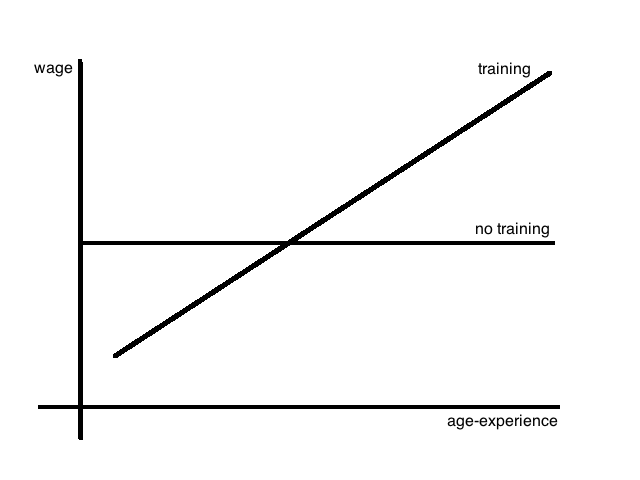
\includegraphics[width=4in, height=3in]{plot14.png}
\end{figure}
\end{center}

An area comparison ratio will give you the return of the training investment.
\begin{itemize}
\item Why does training happens when you are young?
    \begin{itemize}
    \item If you want to acquire skills you may want to do it know in order to maximize the gain from that acquisition.
    \end{itemize}
\item How does learning by doing looks like (happen)?
\end{itemize}

\begin{center}
\begin{figure}[H] 
\caption{}
\centering
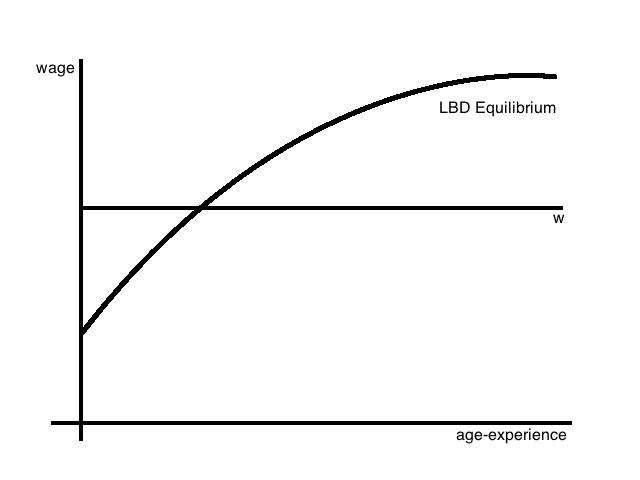
\includegraphics[width=4in, height=3in]{plot15.png}
\end{figure}
\end{center}

\textbf{Who pays for the training?}

Clearly, this depends on the market structure and on the kind of training people receive.

There are 4 types of training:
\begin{itemize}
\item firm specific
\item industry specific
\item occupational specific
\item general training
\end{itemize}

\begin{itemize}
\item If the market is competitive general training raises productivity in all markets. Then, no firm will be willing to pay for that employee's training.
\item If there is a competitive industry, the worker will face a higher uncertainty than in the general case and it is uncertain who is paying for the training.
\item firm specific: firm pays.
\end{itemize}

\textbf{Why is there job specialization}

``Division of labor is limited by the extension of the economy''. Adam Smith

Is development leading to more specialization or is specialization leading to more development? You may argue in both senses.

Two fundamental approaches for trying to understand why people differ.

\begin{enumerate}[1.]
\item Roy model of specialization and comparative advantage.
    \begin{itemize}
    \item take differences as given
    \end{itemize}
\end{enumerate}

\textbf{Is this arguable?}

\begin{enumerate}[1.]
\item Yes, people become different too. How? Training, learning by doing, human capital investment, etc.
\item Becker model: attack a problem in which individuals are identical ex-ante.
\end{enumerate}

\textbf{Assumptions}:

\begin{itemize}
\item identical individuals ex-ante
\item specialization in different skills or tasks
\item cooperation among specialists to produce widgets
\item cooperation is in teams (not only a firm, within a firm)
\item there are m tasks
\item investment in task specific skills (no dynamics)
\item $T$ hours available per individual
\item $h$ time spent investing in this task
\item $H = g(h)$ investment function, where $g'(\cdot)>0$ and $g'' \leq 0$.
\end{itemize}

\textbf{Think}: it pays to develop different kind of skills. Why? increasing returns on doing it.

\textbf{$y$ is the output produced}: It is proportional to the effective labor input (works spent working times productivity).

\begin{equation*}
Y = \overbrace{\alpha}^{\text{productivity of economy}} \cdot \underbrace{l \cdot H}_{\text{effective labor}}
\end{equation*}

$g(n,A_c,A_{N_c}) \implies$ complementarity with other individuals, etc. is brought by the shape of $g$.

Time can be allocated working or spending in human capital:
\begin{equation*}
\boxed{l + h = T}
\end{equation*}

The problem that any agent faces is:
\begin{equation*}
\underset{l,h}{\text{MAX}} \quad \{Y = \alpha \cdot l \cdot g(h)\}
\end{equation*}

\textbf{F.O.C.s}
\begin{equation*}
[l]: \alpha g(h) = \lambda \quad [h]: \alpha \cdot l \cdot g'(h) = \lambda \Leftrightarrow \boxed{l^* = \frac{g(h)}{g'(h)}} \boxed{h^* = T - \frac{g(h)}{g'(h)}}
\end{equation*}

Suppose that $g(h) = c h^{\theta} \quad  0 \leq \theta \leq 1$, where $c(A_{N_c},A_c)$, etc.

Then:
\begin{equation*}
\boxed{l^* = \frac{h^*}{\theta}}
\end{equation*}
and
\begin{equation*}
\boxed{l^* + h^* = T}
\end{equation*}

\begin{equation*}
\boxed{l^* = \frac{1}{1+\theta} \cdot T} \\
\boxed{h^* = \frac{\theta}{1+\theta} \cdot T}
\end{equation*}

In equilibrium, what is the output?

\begin{equation*}
Y^* = \alpha \cdot l^* \cdot g(h^*) = \frac{\alpha \cdot g(h^*)}{g'(h^*)} \cdot g(h^*) = \boxed{\frac{\alpha \cdot g^2(h^*)}{g'(h^*)} = Y^*}
\end{equation*}

Notice that there are increasing returns in investing in specialization.
If $g(h)=ch^{\theta}$, then:
\begin{equation*}
Y^* = \frac{\alpha c}{(1+\theta)^{\theta+1}} \rightarrow \quad \text{better to be more able}
\end{equation*}

If $\theta = 1$,
\begin{equation*}
\boxed{Y^* = \frac{\alpha c}{4} T^2}
\end{equation*}

\begin{itemize}
\item Increasing in $T$; double your time, more than double your output.
\item This is why you don't want to diversify, you want to concentrate.
\end{itemize}

To show more clearly the benefits of specialization, let's deal with a double task (independent) case.

\begin{itemize}
\item Tasks: $y_1, y_2$
\item investment functions: $g(h_1), g(h_2)$
\item Restrictions: \begin{align*}
                        h_1 + l_1 &= t_1 \\
                        h_2 + l_2 &= t_2 \\
                        t_1 + t_2 &= T
                    \end{align*}
\end{itemize}

``Obviously'':
\begin{align*}
Y^*_1 = \frac{\alpha_1 c_1}{\theta_1} \cdot [\frac{\theta_1}{1+\theta_1}]^{1+\theta_1} \cdot {t^{1+\theta_1}} \quad Y^*_2 = \frac{\alpha_2 c_2}{\theta_2} [\frac{\theta_2}{1+\theta_2}]^{1+\theta_2} \cdot t^{1+\theta_2}_2
\end{align*}

Now, suppose $t_i = \frac{T}{2}$, for $i = 1,2$

\textbf{What is the effect of dividing time?}

$Y^* = [ \quad ] \frac{T^{1+\theta}}{2^{1+\theta}}$; output decreases more than half.

Suppose that the joint production function, $\phi = f(Y_1,Y_2)$ is leontief (la favorita del skoto) $\phi(Y_1,Y_2) = min (Y_1,Y_2)$, then $Y^*_1 = Y^*_2$.

This will cause people to put a lot of time to the thing they are not good at.

If $\alpha_1 = \alpha_2, c_1 = c_2, \theta_1 = \theta_2$, is same for everyone, then $t^*_1 = t^*_2$ obviously $Y^*_1 = Y^*_2$ (leontief)

Then:
\begin{equation*}
Y^* = Y^*_1 = Y^*_2 = \frac{\alpha c}{4}(\frac{T}{2})^2 = \boxed{\frac{\alpha c T^2}{16} = Y^*}
\end{equation*}

\begin{itemize}
\item If somebody needs to produce in fixed properties, they suffer a lot when they specialize.
\end{itemize}

Suppose $\alpha_1 = \alpha_2 = \alpha, \theta_1 = \theta_2 = \theta$ and $c_1 \neq c_2$ s.t. $c_1 > c_2$, then
$t_1 < t_2$.

More productive in task 1, you allocate less time in it. If $\theta = 1$ and $c_1 = 2c_2 \implies t_1 = \frac{t_2}{\sqrt{2}}$.

Finally, if there are $m$ tasks and $\phi =$ min $\{y_1,\dots,y_m\}$:
\begin{equation*}
\boxed{Y^*_i = [\cdot] \frac{t^2}{m^2}}
\end{equation*}

\begin{itemize}
\item \framebox[1.1\width]{What have we learned today? (Nothing), there are huge gains from specialization}
\end{itemize}

\begin{itemize}
\item Entrepreneur coordinates people
\end{itemize}

\textbf{Coordination Costs}
\begin{itemize}
\item communication
\item complementarity
\item cost function of coordination is increasing in the number of members the team has
\end{itemize}

\begin{itemize}
\item \textbf{Model}
\end{itemize}

$n = \#$ of members = $\frac{m}{s}$, where $s$ is $\#$ of independent tasks

cost function: \quad $c(n), c'(n) > 0, c''(n) > 0$

$n(n-1)$ possible interactions

$I = $ per capita income = $y(\frac{m}{n}) - c(n)$
\begin{align*}
\frac{dI}{dn} = \frac{dy}{dn} - c'(n) > 0, \quad \forall n \leq m\ \ N < m
\end{align*}

$N$ = numbers of individuals available (number of the market)

$s = \frac{m}{N} > 1 \rightarrow$ in this case division of labor is limited by extent of the market.

\begin{enumerate}[1.]
\item $\checkmark$ prior
\item $y'(n) < c'(n)$ all $n > 1$ (coordination costs are too big) (inefficient)
\item Division of labor limited by extent of the economy \\
\begin{align*}
&y'(n) > c'(n) \quad &\text{at the beginning} \\
&c'(n) > y'(n) \quad &\text{at the end ($c'(n)$ convex)}
\end{align*}
In this case there is an interior solution.
\begin{align*}
\underset{h}{\text{MAX}} \quad &I = y(n) - c(n) \quad 1 < n^* < m \\
&\text{FOC} \quad y'(n) = c'(n) \quad \text{$\#$ teams} = m \\
&\text{SOC} \quad c''(n) = y''(n) > 0
\end{align*}
\end{enumerate}

\begin{itemize}
\item Household
\end{itemize}

2 members
Household markets, $m = 2$. \\
How do you explain that women are always in the market place
\begin{enumerate}[1.]
\item Roy-differences
\item Discrimination
\end{enumerate}

\end{document} 